\section{Question 2}

\subsection{Question}
Download the TimeMaps for each of the target URIs.  We'll use the mementoweb.org 
Aggregator, so for example:\\

URI-R = http://www.cs.odu.edu/\\

URI-T = http://mementoweb.org/timemap/link/http://www.cs.odu.edu/\\

You could use the cs.odu.edu aggregator:\\

URI-T = http://mementoproxy.cs.odu.edu/aggr/timemap/link/1/http://www.cs.odu.edu/\\

But be sure to say which aggregator you use -- they are likely to give
different answers.\\

Create a histogram of URIs vs. number of Mementos (as computed from
the TimeMaps).  For example, 100 URIs with 0 Mementos, 300 URIs
with 1 Memento, 400 URIs with 2 Mementos, etc.\\

See: http://en.wikipedia.org/wiki/Histogram\\

Note that the TimeMaps can span multiple pages.  Look for links like:\\

<http://mementoweb.org/timemap/link/1000/http://www.cnn.com/>;rel="timemap"; 
type="application/link-format"; from ="Sun, 08 Jul 2001 21:30:54 GMT"\\

This indicates another page of the TimeMap is available.  There can be 
many pages to a TimeMap.\\

\subsection{Resources}
\begin{itemize}
\item R: \url{http://www.cs.odu.edu/~sainswor/uploads/Teaching/cs595f13-R.pdf}
\end{itemize}

\subsection{Answer}
Using a simple python script to get the timemaps and then parse the results, traveling down the rabbit hole if the target uri has more than 1000 mementos, was done with the following code.

\lstinputlisting[language=Python, caption={mementofinder.py}, label=listing:mementofinder]{q2/mementofinder.py}

And the results of running the python code in Listing \ref{listing:mementofinder}. A log scale was used along the y axis to show more detail among the results. 

\begin{figure}[h!]
\centering
\label{fig:hist_ss}
\fbox{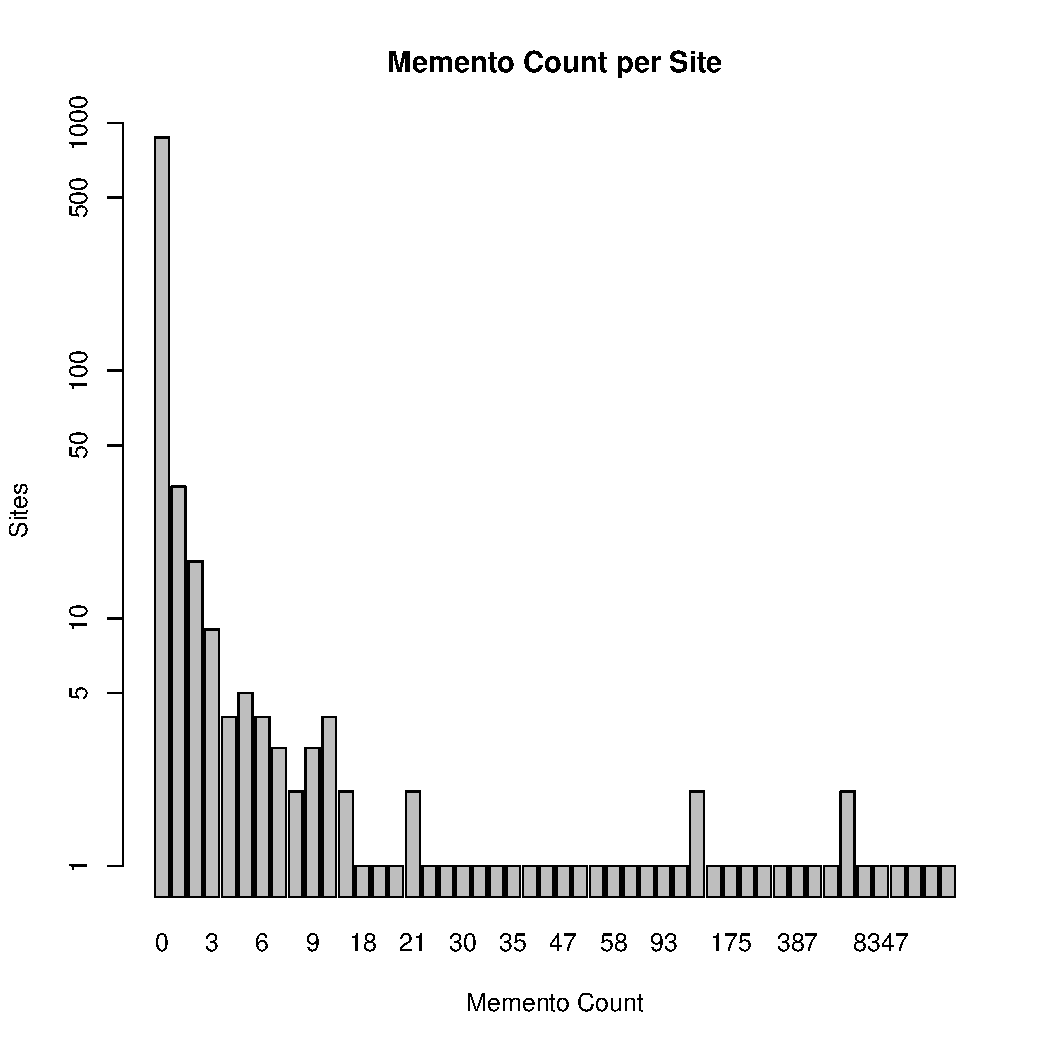
\includegraphics[scale=.75]{q2/hist.pdf}}
\caption{Histogram of Site Mementos}
\end{figure}
